\section{Структура FILE}

\begin{lstlisting}[caption=Описание структуры FILE (\_\_sFILE),label=lst:FILEstruct1]
typedef struct __sFILE {
	unsigned char *_p;	/* current position in (some) buffer */
	int _r;	/* read space left for getc() */
	int _w;	/* write space left for putc() */
	short _flags;	/* flags, below; this FILE is free if 0 */
	short _file;	/* fileno, if Unix descriptor, else -1 */
	struct __sbuf _bf; /* the buff (at least 1 byte, if !NULL) */
	int _lbfsize;	/* 0 or -_bf._size, for inline putc */
	/* operations */
	void *_cookie;	/* cookie passed to io functions */
	int (* _Nullable _close)(void *);
	int (* _Nullable _read)(void *, char *, int);
	fpos_t (* _Nullable _seek)(void *, fpos_t, int);
	int (* _Nullable _write)(void *, const char *, int);
	/* separate buffer for long sequences of ungetc() */
	struct __sbuf _ub;	/* ungetc buffer */
	struct __sFILEX *_extra; /* additions to FILE to not break ABI */
	int _ur;	/* saved _r when _r is counting ungetc data */
	/* tricks to meet minimum requirements even when malloc() fails */
	unsigned char _ubuf[3];	/* guarantee an ungetc() buffer */
	unsigned char _nbuf[1];	/* guarantee a getc() buffer */
	/* separate buffer for fgetln() when line crosses buffer boundary */
	struct __sbuf _lb;	/* buffer for fgetln() */
	/* Unix stdio files get aligned to block boundaries on fseek() */
	int _blksize;	/* stat.st_blksize (may be != _bf._size) */
	fpos_t _offset;	/* current lseek offset (see WARNING) */
} FILE;
\end{lstlisting}

\subsection*{Cравнение полей реализаций структуры FILE (BSD и glibc)}

Обе структуры реализуют cтруктуру типа FILE, определенной в файле стандартных описаний <<stdio.h>>.

Наиболее распространены две реализации:
\begin{itemize}
	\item \texttt{\_\_sFILE} — используется в BSD-системах (FreeBSD, macOS),
	\item \texttt{\_IO\_FILE} — используется в GNU Libc (Linux).
\end{itemize}

\begin{longtable}{|>{\raggedright\arraybackslash}p{4.5cm}|>{\raggedright\arraybackslash}p{5.5cm}|>{\raggedright\arraybackslash}p{5.5cm}|}
	\hline
	\textbf{Назначение} & \textbf{BSD (\_\_sFILE)} & \textbf{GNU (\_IO\_FILE)} \\
	\hline
	Указатель на текущую позицию в буфере & \texttt{unsigned char *\_p} & \texttt{char *\_IO\_read\_ptr}, \texttt{char *\_IO\_write\_ptr} \\
	\hline
	Доступные байты для чтения & \texttt{int \_r} (read count) & Разница между \texttt{\_IO\_read\_end} и \texttt{\_IO\_read\_ptr} (оба типа \texttt{char *}) \\
	\hline
	Доступные байты для записи & \texttt{int \_w} (write count) & Разница между \texttt{\_IO\_write\_end} и \texttt{\_IO\_write\_ptr} (оба типа \texttt{char *}) \\
	\hline
	Буфер & 
	\texttt{struct \_\_sbuf \_bf (Поля: \newline unsigned char *\_base;  \newline int \_size;)} & 
	\texttt{char *\_IO\_buf\_base}, \texttt{char *\_IO\_buf\_end} \\
	\hline
	Номер дескриптора & \texttt{short \_file} & \texttt{int \_fileno} \\
	\hline
	Размер системного блока & \texttt{int \_blksize} & \texttt{int \_blksize} \\
	\hline
	Смещение в файле & \texttt{fpos\_t \_offset} & \texttt{off64\_t \_old\_offset} \\
	\hline
	Флаги & \texttt{short \_flags} & \texttt{int \_flags}, \texttt{int \_flags2} \\
	\hline
	Минимальные буферы & \texttt{unsigned char \_ubuf[3]}, \texttt{unsigned char \_nbuf[1]} & \texttt{char \_shortbuf[1]}, \newline\texttt{int \_cur\_column} \\
	\hline
	Механизм блокировки & Отсутствует явно & \texttt{void *\_lock} — указатель на мьютекс \\
	\hline
	Системные функции ввода-вывода & 
	Указатели на функции:
	\begin{itemize}
		\item \texttt{int (*\_read)(void *, char *, int);}
		\item \texttt{int (*\_write)(void *, const char *, int);}
		\item \texttt{fpos\_t (*\_seek)(void *, fpos\_t, int);}
		\item \texttt{int (*\_close)(void *);}
	\end{itemize}
	Контекст: \texttt{void *\_cookie} & 
	Вызов через vtable: \texttt{struct \_IO\_jump\_t *\_vtable}
	\begin{itemize}
		\item \texttt{ssize\_t (*\_IO\_read)(...)}
		\item \texttt{ssize\_t (*\_IO\_write)(...)}
		\item \texttt{off64\_t (*\_IO\_seekoff)(...)}
		\item и др.
	\end{itemize} \\
	\hline
	Поддержка \texttt{ungetc()} -- откат чтения & \texttt{struct \_\_sbuf \_ub}; \newline\texttt{int \_ur} & \texttt{char *\_IO\_backup\_base}, \texttt{\_IO\_save\_base}, \texttt{\_IO\_save\_end} \\
	\hline
	Поддержка \texttt{fgetln()} & \texttt{struct \_\_sbuf \_lb} & Нет аналога \\
	\hline
	Расширения & \texttt{void *\_extra} & \texttt{struct \_IO\_marker *\_markers}, \newline\texttt{struct \_IO\_FILE *\_chain} \\
	\hline
\end{longtable}

\newpage
\section{Программа №1}

\subsection*{Однопоточная реализация}
\begin{lstlisting}[caption=Первая программа (однопоточная),label=lst:FILEstruct]
#include <stdio.h>
#include <stdlib.h>
#include <fcntl.h>
#define FILE_NAME 	"../alphabet.txt"
#define BUFF_SIZE 	20
#define RED     	"\x1b[31m"
#define GREEN   	"\x1b[32m"
#define RESET   	"\x1b[0m"

int main() {
	int fd = open(FILE_NAME, O_RDONLY);
	if (fd == -1) {
		perror("open");
		exit(EXIT_FAILURE);
	}
	FILE *fs1 = fdopen(fd, "r");
	char buf1[BUFF_SIZE];
	setvbuf(fs1, buf1, _IOFBF, BUFF_SIZE); 
	FILE *fs2 = fdopen(fd, "r");
	char buf2[BUFF_SIZE];
	setvbuf(fs2, buf2, _IOFBF, BUFF_SIZE);
	int rc1 = 1, rc2 = 1;
	while (rc1 == 1 || rc2 == 1) {
		char c;
		rc1 = fscanf(fs1, "%c", &c);
		if (rc1 == 1)
			fprintf(stdout, RED "%c" RESET, c);
		rc2 = fscanf(fs2, "%c", &c);
		if (rc2 == 1)
			fprintf(stdout, GREEN "%c" RESET, c);
	}
	fclose(fs1); 
	fclose(fs2);
	exit(EXIT_SUCCESS);
}
\end{lstlisting}

\newpage
\begin{figure}[h!] 
	\centering
	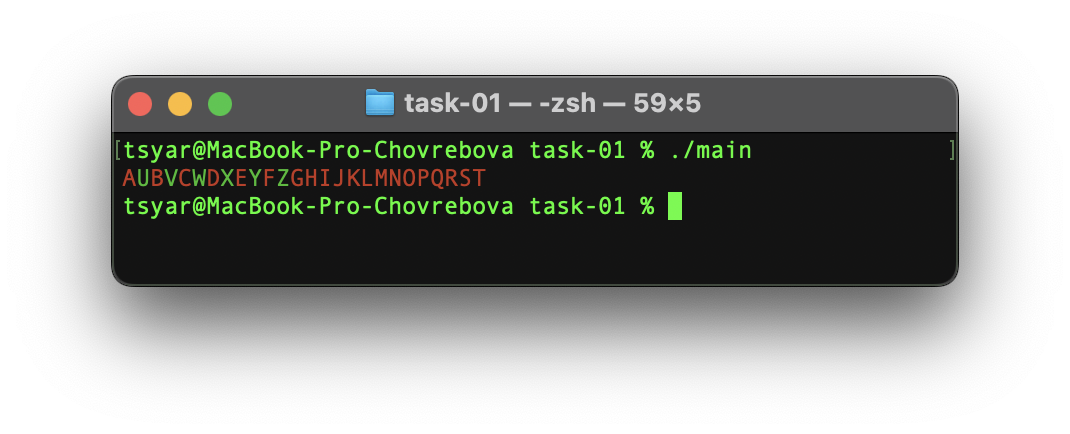
\includegraphics[width=1.0\textwidth]{./img/first-01.png}
	\caption{Результат работы программы первой однопоточной программы}
	\label{fig:1}
\end{figure}

\subsubsection*{Анализ работы программы}

Программа считывает информацию из файла «alphabet.txt», который содержит англиский алфавит -- строку символов. В результате своей работы программа при помощи двух буферов посимвольно выводит считанные символы в стандартный поток вывода stdout.

Во время выполнения программы вызывается системный вызов \textbf{open()}, который создает новый файловый дескриптор для открытого в режиме <<только для чтения>> файла <<alphabet.txt>>  и возвращает созданный файловый дескриптор из системной таблицы открытых процессом файлов.

Дважды вызывается функция \textbf{fdopen()}, которая связывает поток ввода-вывода со существующим файловым дескриптором. Каждый вызов \textbf{fdopen()} создает отдельную структуру \_\_sFILE (BSD) либо \_IO\_FILE (Linux, GNU), связанную с одним и тем же файловым дескриптором, и возвращает указатель типа FILE на эту структуру. Таким образом, получаются два независимых потока, использующих один и тот же дескриптор файла, но имеющих собственные буферы.

Далее с помощью функции \textbf{setvbuf()} изменяется тип буферизации для \textbf{fs1} и \textbf{fs2} на полную буферизацию -- при полной буферизации данные хранятся в буфере и записываются в файл только тогда, когда буфер полностью заполнен; также явно задается размер буфера \textbf{BUFF\_SIZE} равный 20.

В цикле происходит считывание символов из файла с помощью функции  \textbf{fscanf()}.
При первом вызове  \textbf{fscanf()} данные записываются в буфер  \textbf{buf1}: первые 20 символов из файла, а указатель текущей позиции в файле (\textbf{f\_pos}) перемещается на позицию, соответствующую следующему байту после последнего считанного.
При следующем вызове  \textbf{fscanf()} в буфер \textbf{buf2} записываются оставшиеся символы файла, после чего указатель \textbf{f\_pos} перемещается в конец файла.

При выводе содержимого буферов \textbf{buf1} и \textbf{buf2} с помощью вызова \textbf{fprintf()} символы считываются поочерёдно из двух буферов. В результате после символа 'A' из первого буфера сразу следует символ 'U' из второго буфера.

\begin{figure}[h!] 
	\centering
	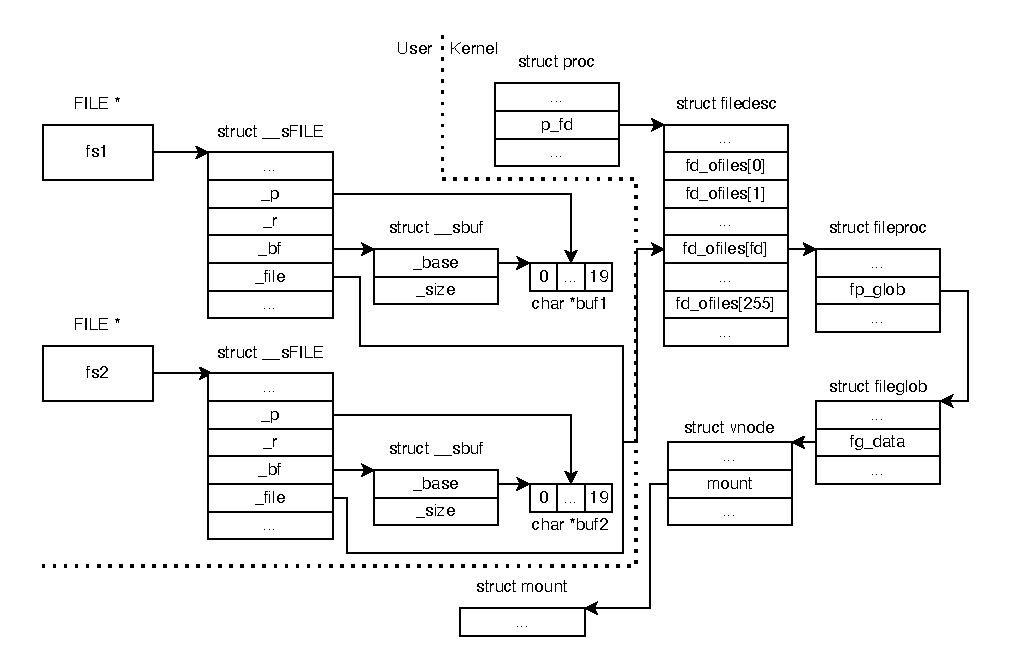
\includegraphics[width=1.1\textwidth]{./img/first-01.pdf}
	\caption{Связь структур файловой подсистемы (BSD, Darwin-XNU)}
	\label{fig:2}
\end{figure}

\newpage
\begin{figure}[h!] 
	\centering
	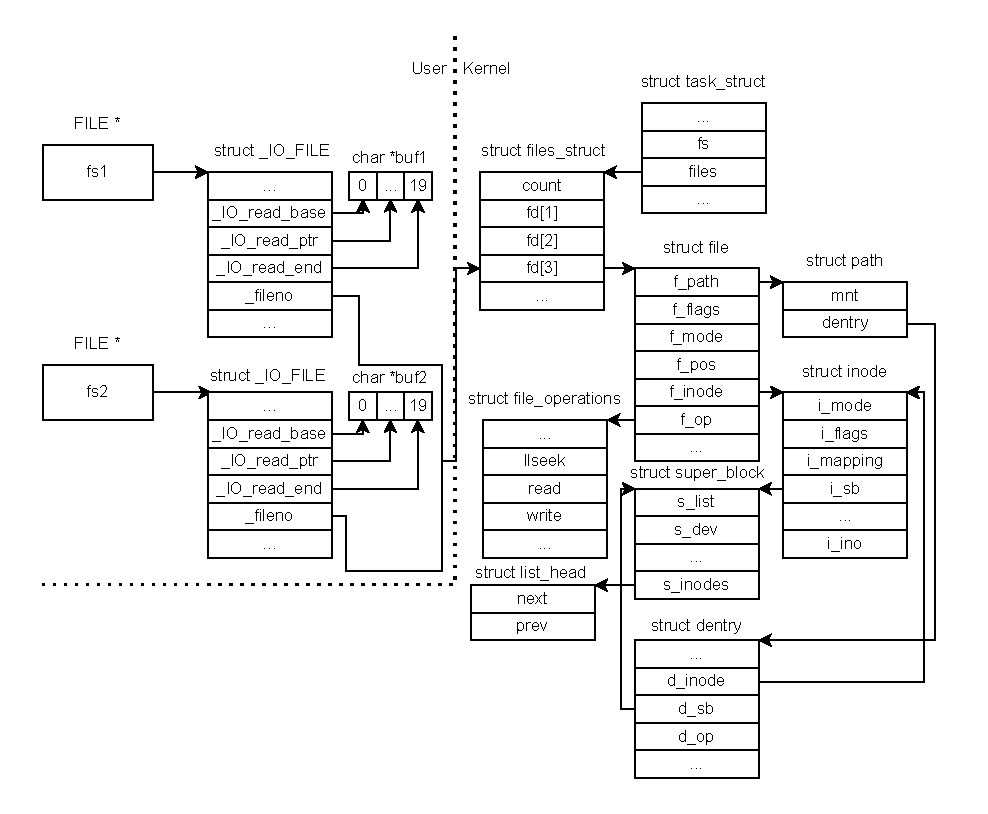
\includegraphics[width=1.03\textwidth]{./img/first-02.pdf}
	\caption{Связь структур файловой подсистемы Linux}
	\label{fig:3}
\end{figure}

\subsection*{Многопоточная}
\begin{lstlisting}[caption=Первая программа (многопоточная),label=lst:FILEstruct11]
#include <stdio.h>
#include <stdlib.h>
#include <fcntl.h>
#include <pthread.h>
#include <unistd.h>

#define FILE_NAME 	"../alphabet.txt"
#define BUFF_SIZE    20

#define RED         "\x1b[31m"
#define GREEN       "\x1b[32m"
#define RESET       "\x1b[0m"

void *fileReader(void *args) {
	FILE *fs = (FILE *)args;
	int rc = 1;
	char c;
	while (rc == 1) {
		if ((rc = fscanf(fs, "%c\n", &c)) == 1)
			fprintf(stdout, GREEN "%c" RESET, c);
	}
	return NULL;
}

int main(void) {
	int fd = open(FILE_NAME, O_RDONLY);
	if (fd == -1) {
		perror("open");
		exit(EXIT_FAILURE);
	}
	FILE *fs1 = fdopen(fd, "r");
	char buf1[BUFF_SIZE];
	setvbuf(fs1, buf1, _IOFBF, BUFF_SIZE);
	FILE *fs2 = fdopen(fd, "r");
	char buf2[BUFF_SIZE];
	setvbuf(fs2, buf2, _IOFBF, BUFF_SIZE);
	pthread_t thread;
	int prc;
	if ((prc = pthread_create(&thread, NULL, fileReader, (void *)fs2)) != 0) {
		fclose(fs1); fclose(fs2);
		fprintf(stderr, "pthread_create failed: %s\n", strerror(prc));
		exit(EXIT_FAILURE);
	}
	int rc = 1;
	char c;
	while (rc == 1) {
		rc = fscanf(fs1, "%c\n", &c);
		if (rc == 1)
			fprintf(stdout, RED "%c" RESET, c);
	}
	if (pthread_join(thread, NULL) != 0) {
		fclose(fs1); fclose(fs2);
		fprintf(stderr, "pthread_create failed: %s\n", strerror(prc));
		exit(EXIT_FAILURE);
	}
	fclose(fs1);
	fclose(fs2);
	exit(EXIT_SUCCESS);
}
\end{lstlisting}

\begin{figure}[h!] 
	\centering
	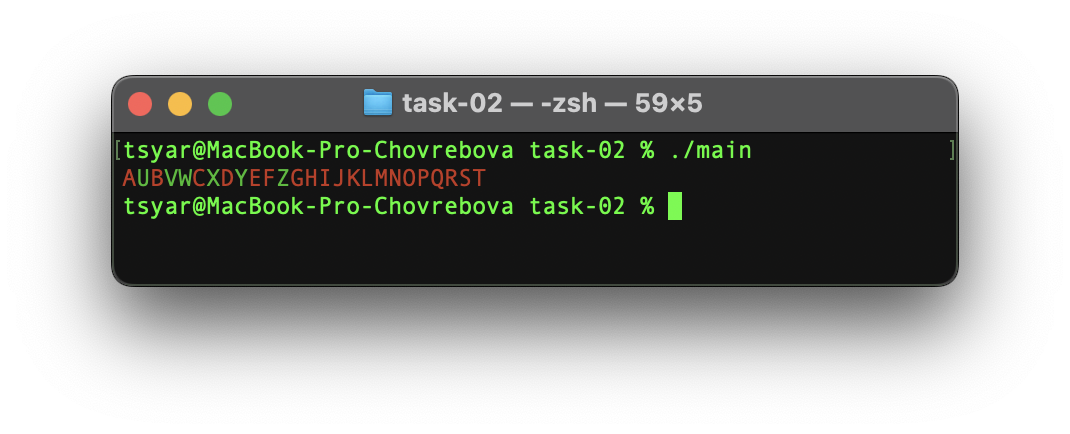
\includegraphics[width=1.0\textwidth]{./img/first-02.png}
	\caption{Результат работы первой многопоточной программы}
	\label{fig:4}
\end{figure}

В многопоточной реализации программы вывод зависит от планирования потоков в системе. Первый поток чаще всего успевает отработать первым, из-за временных затрат на создание второго потока.

\newpage
\section{Программа №2}

\subsection*{Однопоточная реализация}

\begin{lstlisting}[caption=Вторая программа (однопоточная),label=lst:FILEstruct111]
#include <stdlib.h>
#include <fcntl.h>
#include <unistd.h>

#define FILE_NAME "../alphabet.txt"
#define CHAR_SIZE sizeof(char)
#define BUFF_SIZE 32 * CHAR_SIZE

int main() {
	int fd1 = open(FILE_NAME, O_RDONLY);
	if (fd1 == -1) {
		write(STDERR_FILENO, "error: open fd1\n", BUFF_SIZE);
		exit(EXIT_FAILURE);
	}
	int fd2 = open(FILE_NAME, O_RDONLY);
	if (fd2 == -1) {
		write(STDERR_FILENO, "error: open fd2\n", BUFF_SIZE);
		close(fd1);
		exit(EXIT_FAILURE);
	}
	int rc1 = 1, rc2 = 1;
	char c;
	while (rc1 == 1 || rc2 == 1) {
		rc1 = read(fd1, &c, CHAR_SIZE);
		if (rc1 == 1)
			write(STDOUT_FILENO, &c, CHAR_SIZE);
		rc2 = read(fd2, &c, 1);
		if (rc2 == 1)
			write(STDOUT_FILENO, &c, CHAR_SIZE);
	}
	write(STDOUT_FILENO, "\n", 1);
	close(fd1);
	close(fd2);
	exit(EXIT_SUCCESS);
}
\end{lstlisting}

\begin{figure}[h!] 
	\centering
	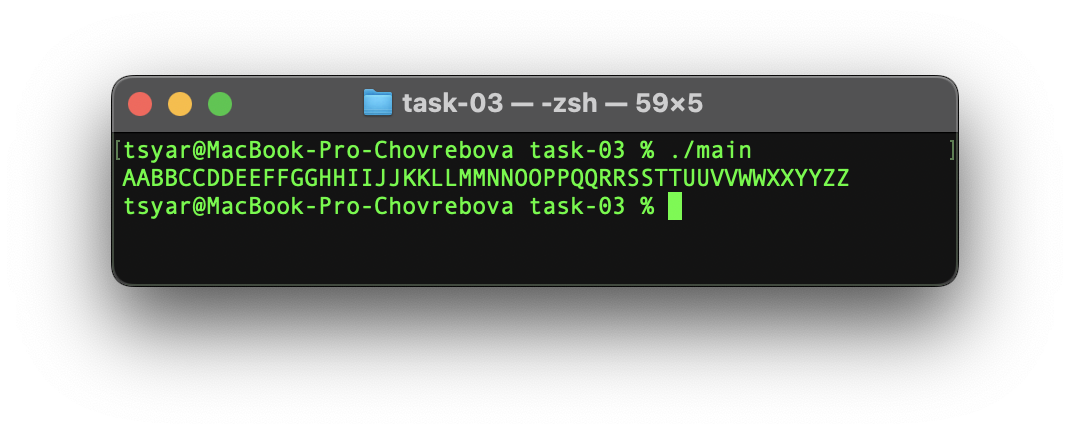
\includegraphics[width=1.0\textwidth]{./img/second-01.png}
	\caption{Результат работы программы}
	\label{fig:111}
\end{figure}

\subsubsection*{Анализ работы программы}

Во время выполнения программы дважды вызывается системный вызов \textbf{open()}, который создает новый файловый дескриптор для открытого в режиме <<только для чтения>> файла <<alphabet.txt>> и возвращает созданный файловый дескриптор из системной таблицы открытых файлов процесса. Таким образом, создаются два независимых файловых дескриптора, указывающих на один и тот же файл. Для каждого дескриптора ядро создаёт отдельную структуру \textbf{struct file}, которая, помимо прочего, содержит поле \textbf{f\_pos} — текущее смещение в файле. Поскольку дескрипторы независимы, их смещения (\textbf{f\_pos}) также управляются независимо.

Далее в цикле поочередно считываются символы из файла и выводятся в стандартный потока вывода с использованием системного вызова \textbf{write()}. В результате каждый символ файла выводится дважды -- поскольку оба дескриптора читают файл с начала, независимо друг от друга.

\begin{figure}[h!] 
	\centering
	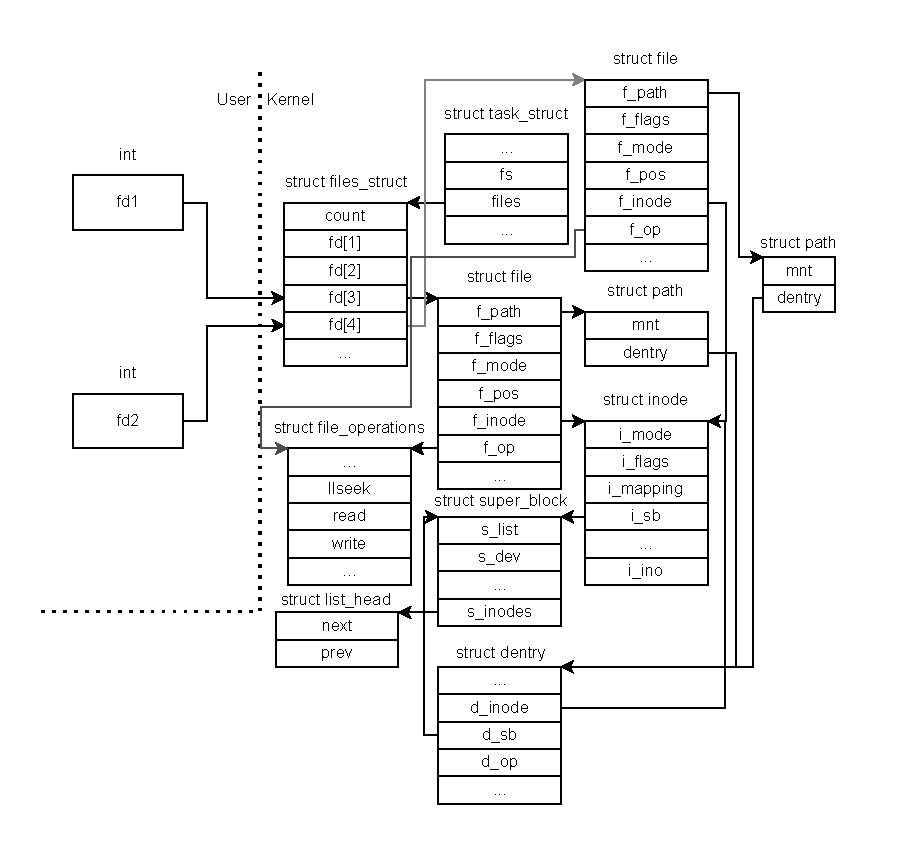
\includegraphics[width=1.03\textwidth]{./img/second.pdf}
	\caption{Связь структур файловой подсистемы Linux}
	\label{fig:33}
\end{figure}
\newpage

\subsection*{Многопоточная реализация}
\begin{lstlisting}[caption=Многопоточная программа c двумя дополнительными потоками,label=lst:FILEstruct11111]
#include <fcntl.h>
#include <unistd.h>
#include <pthread.h>

#define FILE_NAME "../alphabet.txt"
#define CHAR_SIZE sizeof(char)
#define BUFF_SIZE 32 * CHAR_SIZE

void *fileReader(void *args) {
	int fd = *(int *)args;
	int rc = 1;
	char c;
	while (rc == 1) {
		rc = read(fd, &c, CHAR_SIZE);
		if (rc == 1)
			write(STDOUT_FILENO, &c, CHAR_SIZE);
	}
	return NULL;
}

int main() {
	int fd1 = open(FILE_NAME, O_RDONLY);
	if (fd1 == -1) {
		write(STDERR_FILENO, "error: open fd1\n", BUFF_SIZE);
		exit(EXIT_FAILURE);
	}
	int fd2 = open(FILE_NAME, O_RDONLY);
	if (fd2 == -1) {
		write(STDERR_FILENO, "error: open fd2\n", BUFF_SIZE);
		close(fd1);
		exit(EXIT_FAILURE);
	}
	pthread_t thread1, thread2;
	int prc1, prc2;
	if ((prc1 = pthread_create(&thread1, NULL, fileReader, &fd1)) != 0) {
		close(fd1); close(fd2);
		write(STDERR_FILENO, "error: pthread1 create\n", BUFF_SIZE);
		exit(EXIT_FAILURE);
	}
	if ((prc2 = pthread_create(&thread2, NULL, fileReader, &fd2)) != 0) {
		close(fd1); close(fd2);
		write(STDERR_FILENO, "error: pthread2 create\n", BUFF_SIZE);
		exit(EXIT_FAILURE);
	}
	if (pthread_join(thread1, NULL)) {
		close(fd1); close(fd2);
		write(STDERR_FILENO, "error: pthread1 join\n", BUFF_SIZE);
		exit(EXIT_FAILURE);
	}
	if (pthread_join(thread2, NULL)) {
		close(fd1); close(fd2);
		write(STDERR_FILENO, "error: pthread2 join\n", BUFF_SIZE);
		exit(EXIT_FAILURE);
	}
	close(fd1);
	close(fd2);
	exit(EXIT_SUCCESS);
}
\end{lstlisting}

\begin{figure}[h!] 
	\centering
	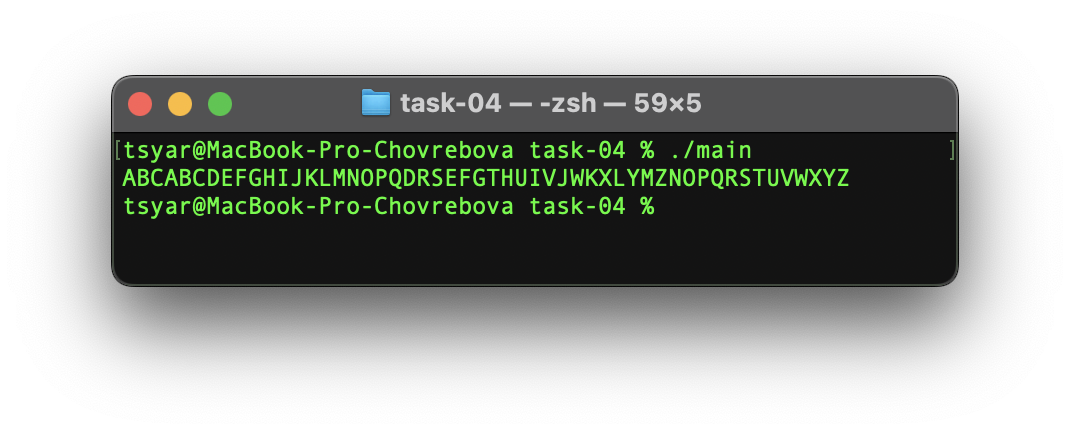
\includegraphics[width=1.0\textwidth]{./img/second-02.png}
	\caption{Результат работы второй многопоточной программы}
	\label{fig:22}
\end{figure}

В многопоточной реализации системный вызов \textbf{open()} также дважды используется для открытия одного и того же файла <<alphabet.txt>> в режиме \textbf{O\_RDONLY}. В результате создаются два независимых файловых дескриптора, каждый из которых связан с собственной структурой \textbf{struct file} в ядре. Эти структуры содержат отдельные значения текущего смещения в файле, что обеспечивает независимое перемещение указателя \textbf{f\_pos} для каждого дескриптора.

Однако, в отличие от однопоточной версии, где чтение из обоих дескрипторов осуществляется последовательно в рамках одного потока, многопоточная реализация организует параллельную обработку с использованием двух дополнительных потоков, создаваемых с помощью \textbf{pthread\_create()}. Каждый поток получает один из файловых дескрипторов в качестве аргумента и выполняет функцию \textbf{fileReader()}, которая реализует цикл чтения по одному символу из файла и немедленного вывода его в стандартный поток вывода (\textbf{STDOUT\_FILENO}) с помощью системного вызова \textbf{write()}.

\begin{lstlisting}[caption=Многопоточная программа c одним дополнительным потоком,label=lst:FILEstruct111211]
#include <fcntl.h>
#include <unistd.h>
#include <pthread.h>

#define FILE_NAME "../alphabet.txt"
#define CHAR_SIZE sizeof(char)
#define BUFF_SIZE 32 * CHAR_SIZE

void *fileReader(void *args) {
	int fd = *(int *)args;
	int rc = 1; char c;
	while (rc == 1) {
		rc = read(fd, &c, CHAR_SIZE);
		if (rc == 1)
			write(STDOUT_FILENO, &c, CHAR_SIZE);
	}
	return NULL;
}

int main() {
	int fd1 = open(FILE_NAME, O_RDONLY);
	if (fd1 == -1) {
		write(STDERR_FILENO, "error: open fd1\n", BUFF_SIZE);
		exit(EXIT_FAILURE);
	}
	int fd2 = open(FILE_NAME, O_RDONLY);
	if (fd2 == -1) {
		write(STDERR_FILENO, "error: open fd2\n", BUFF_SIZE);
		close(fd1);
		exit(EXIT_FAILURE);
	}
	pthread_t thread; int prc;
	if ((prc = pthread_create(&thread, NULL, fileReader, &fd1)) != 0) {
		close(fd1); close(fd2);
		write(STDERR_FILENO, "error: pthread1 create\n", BUFF_SIZE);
		exit(EXIT_FAILURE);
	}
	fileReader(&fd2);
	if (pthread_join(thread, NULL)) {
		close(fd1); close(fd2);
		write(STDERR_FILENO, "error: pthread join\n", BUFF_SIZE);
		exit(EXIT_FAILURE);
	}
	close(fd1); close(fd2);
	exit(EXIT_SUCCESS);
}
\end{lstlisting}

В случае многопоточной программы, алфавит будет выведен 2 раза, но порядок вывода символов заранее предсказать невозможно.

\begin{figure}[h!] 
	\centering
	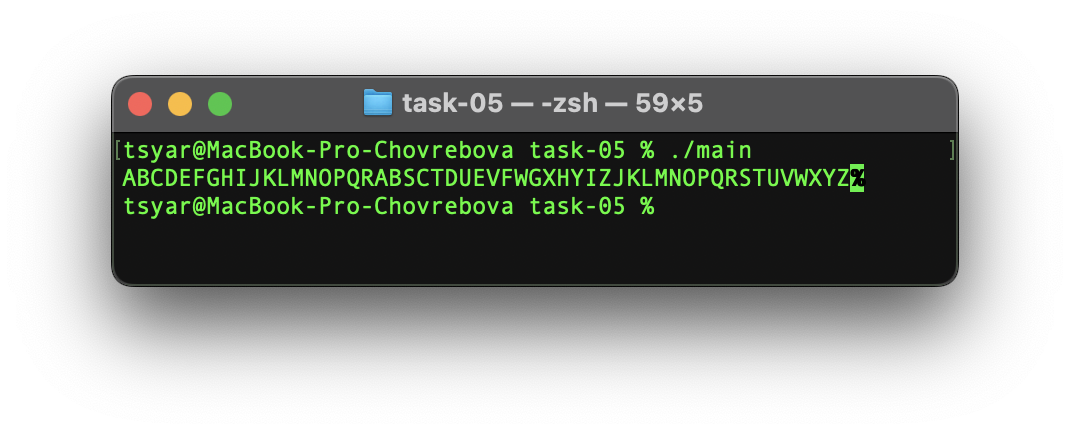
\includegraphics[width=1.0\textwidth]{./img/second-03.png}
	\caption{Результат работы второй многопоточной программы}
	\label{fig:232}
\end{figure}

В данной реализации также создаются два файловых дескриптора, но один обрабатывается в основном потоке, а второй -- в отдельном созданном потоке. Как и ранее, вывод символов может перемешиваться из-за отсутствия синхронизации между потоками.

\newpage
\section{Программа №3}

\subsection*{Однопоточная реализация}

\begin{lstlisting}[caption=Однопоточная программа,label=lst:FILEstruct112211]
#include <stdio.h>
#include <stdlib.h>
#include <fcntl.h>
#include <unistd.h>
#include <sys/stat.h>
#define FILE_OUT "output.txt"

void fileInfo(FILE *f) {
	struct stat statbuf;
	stat(FILE_OUT, &statbuf);
	printf("st_ino: %llu | ", statbuf.st_ino);
	printf("st_size: %d | ", statbuf.st_blksize);
	printf("pos: %ld\n", ftell(f));
}

int main() {
	FILE *f1 = fopen(FILE_OUT, "w");
	fileInfo(f1);
	FILE *f2 = fopen(FILE_OUT, "w");
	fileInfo(f2);
	for (char c = 'A'; c <= 'Z'; c++) {
		if (c % 2) {
			fprintf(f1, "%c", c);
			fileInfo(f1);
		} else {
			fprintf(f2, "%c", c);
			fileInfo(f2);
		}
	}
	fclose(f1);
	fileInfo(f1);
	fclose(f2);
	fileInfo(f2);
	exit(EXIT_SUCCESS);
}
\end{lstlisting}

\begin{figure}[h!] 
	\centering
	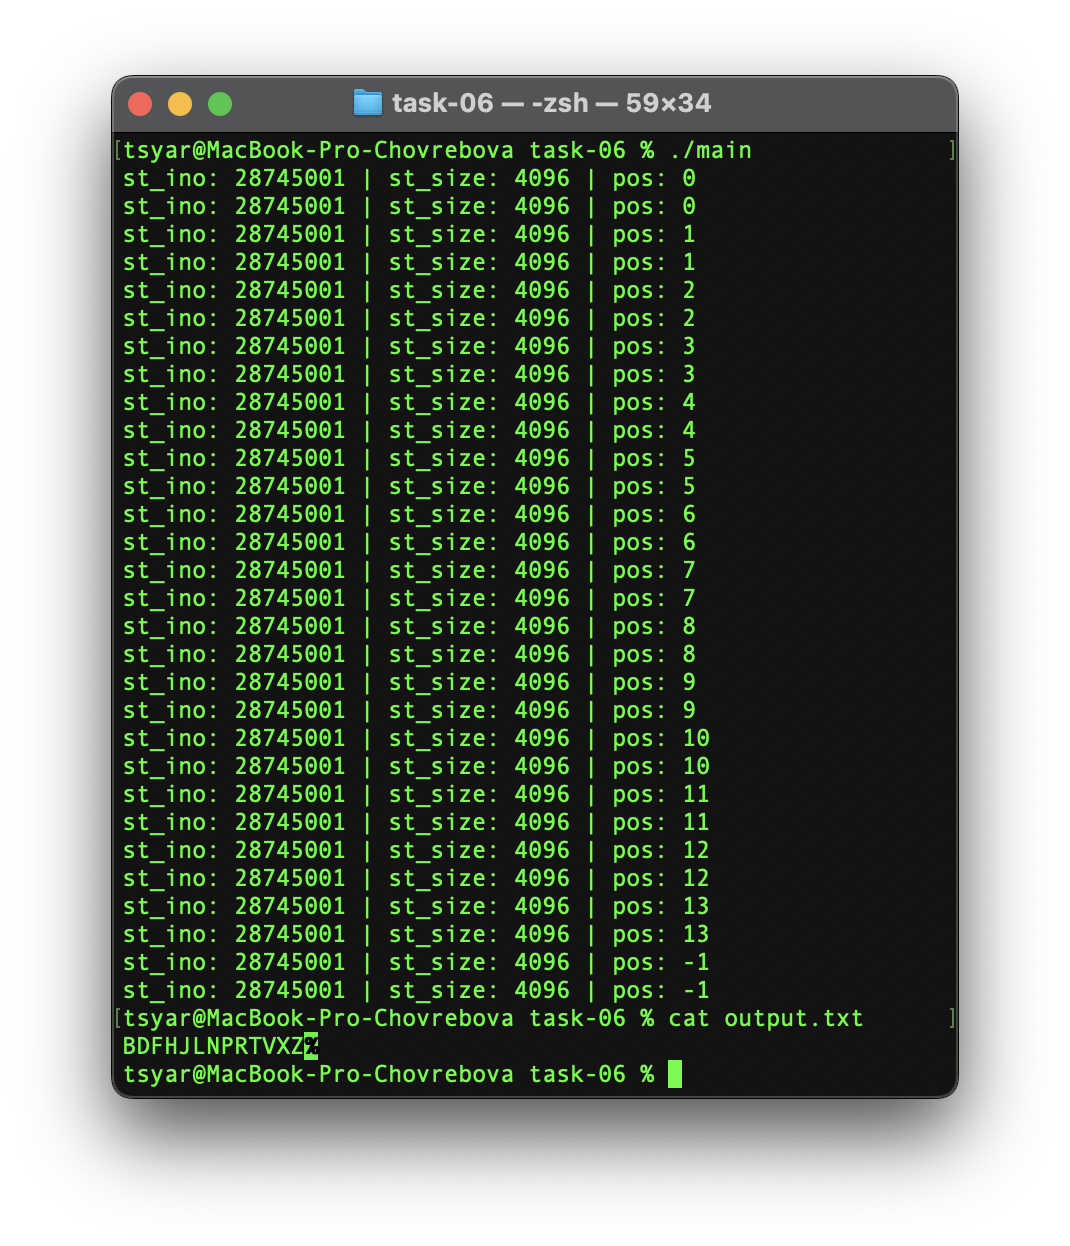
\includegraphics[width=1.0\textwidth]{./img/third-01.png}
	\caption{Результат работы третьей однопоточной программы}
	\label{fig:1111}
\end{figure}

\subsubsection*{Анализ работы программы}

Во время выполнения программы дважды вызывается библиотечная функция \textbf{fopen()} с режимом \texttt{"w"}, что соответствует открытию файла <<output.txt>> только на запись с предварительным обнулением содержимого. Каждый вызов \textbf{fopen()} создает новый файловый дескриптор и инициализирует связанную с ним структуру \textbf{\_IO\_FILE}, управляющую буферизованным вводом-выводом на уровне стандартной библиотеки языка C, и возврашает указатель типа \textbf{FILE} на эту структуру.

Фактическая запись в файл происходит только при вызове \textbf{fflush()} или \textbf{fclose()}, в соответствии с механизмом буферизации стандартной библиотеки.

Во время выполнения программы символы английского алфавита поочередно записываются в разные буферы: нечётные символы направляются в поток f1, чётные -- в поток f2. Однако до момента вызова \textbf{fclose()} содержимое буферов не попадает в файл. После закрытия потока f1 его буфер сбрасывается в файл, и в него записываются нечётные символы. Затем, при закрытии потока f2, его буфер записывается начиная с начала файла (так как файловый дескриптор у потока f2 имел своё смещение), в результате чего данные, записанные через f1, оказываются перезаписанными чётными символами.

\subsection*{Многопоточная}
\begin{lstlisting}[caption=Многопоточная программа c двумя дополнительными потоками,label=lst:FILEstruct11111]
#include <stdio.h>
#include <stdlib.h>
#include <fcntl.h>
#include <pthread.h>
#include <unistd.h>
#include <sys/stat.h>

#define FILE_OUT "output.txt"

struct arg {
	FILE *f;
	int off;
};
pthread_mutex_t mutex = PTHREAD_MUTEX_INITIALIZER;

void fileInfo(FILE *f) {
	struct stat statbuf;
	stat(FILE_OUT, &statbuf);
	pthread_mutex_lock(&mutex);
	printf("st_ino: %llu | ", statbuf.st_ino);
	printf("st_size: %d | ", statbuf.st_blksize);
	printf("pos: %ld\n", ftell(f));
	pthread_mutex_unlock(&mutex);
}

void *fileWriter(void *arg) {
	struct arg *args = (struct arg*) arg;
	for (char c = 'A' + args->off; c <= 'Z'; c+=2) {
		fprintf(args->f, "%c", c);
		fileInfo(args->f);
	}
	return NULL;
}

int main() {
	FILE *f1 = fopen(FILE_OUT, "w");
	fileInfo(f1);
	FILE *f2 = fopen(FILE_OUT, "w");
	fileInfo(f2);
	pthread_t thread1, thread2;
	struct arg arg1 = {.f = f1, .off = 0}; 
	struct arg arg2 = {.f = f2, .off = 1};
	if (pthread_create(&thread1, NULL, fileWriter, &arg1) != 0) {
		perror("error: create thread1");
		fclose(f1); fclose(f2);
		exit(EXIT_FAILURE);
	}
	if (pthread_create(&thread2, NULL, fileWriter, &arg2) != 0) {
		perror("error: create thread2");
		fclose(f1); fclose(f2);
		exit(EXIT_FAILURE);
	}
	pthread_join(thread1, NULL);
	pthread_join(thread2, NULL);
	fclose(f1);
	fileInfo(f1);
	fclose(f2);
	fileInfo(f2);
	exit(EXIT_SUCCESS);
}
\end{lstlisting}

\begin{figure}[h!] 
	\centering
	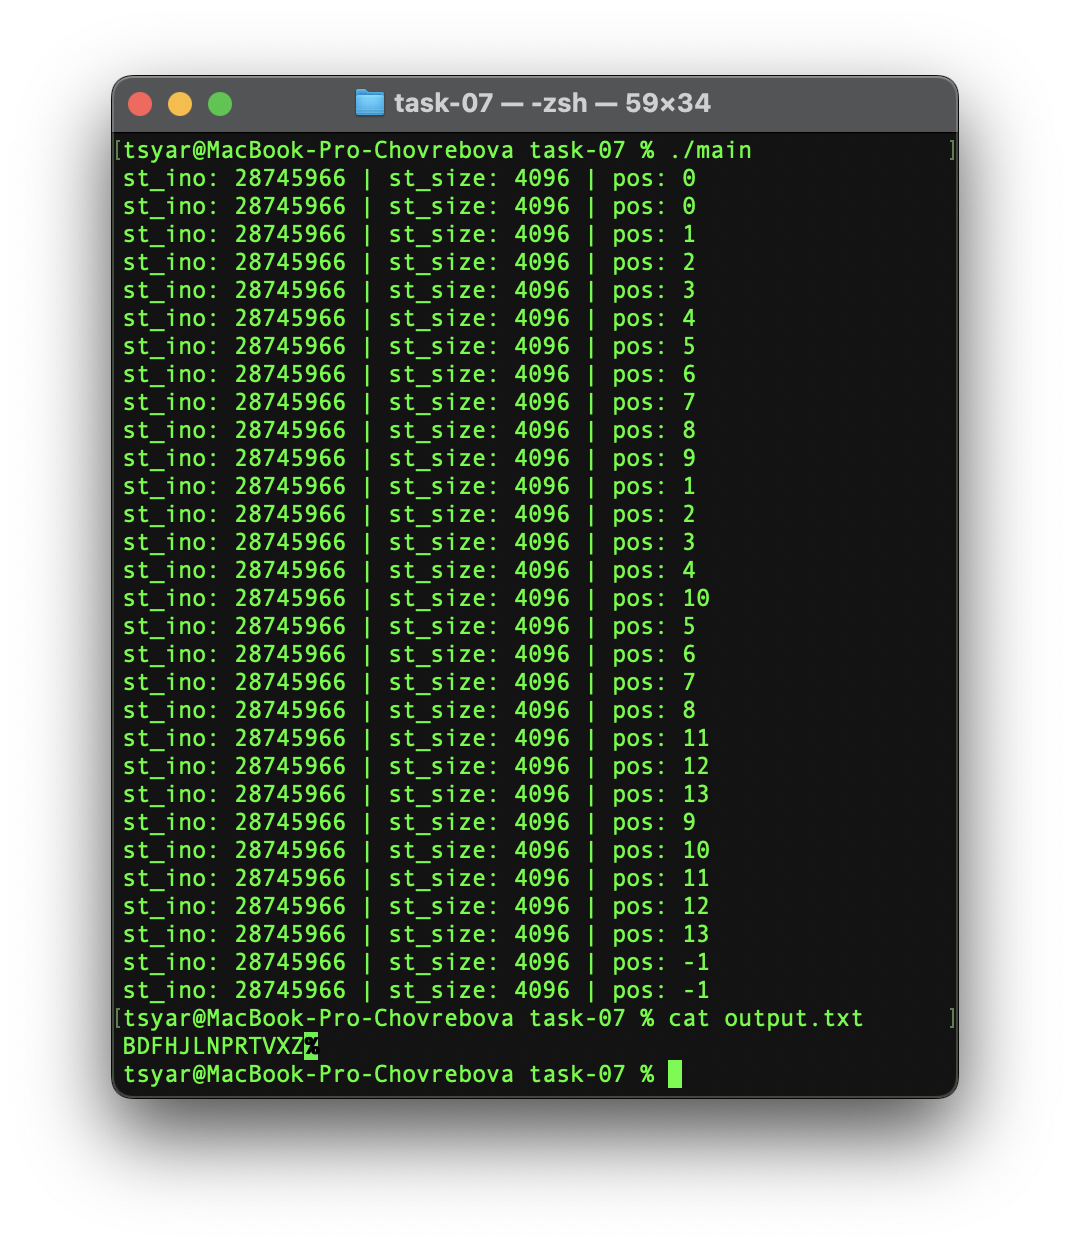
\includegraphics[width=1.0\textwidth]{./img/third-02.png}
	\caption{Результат работы третьей многопоточной программы}
	\label{fig:2222}
\end{figure}

Отличие в работе многопоточной программы от однопоточной в том, что данные записываются в буферы в непредсказуемом порядке.

\begin{figure}[h!] 
	\centering
	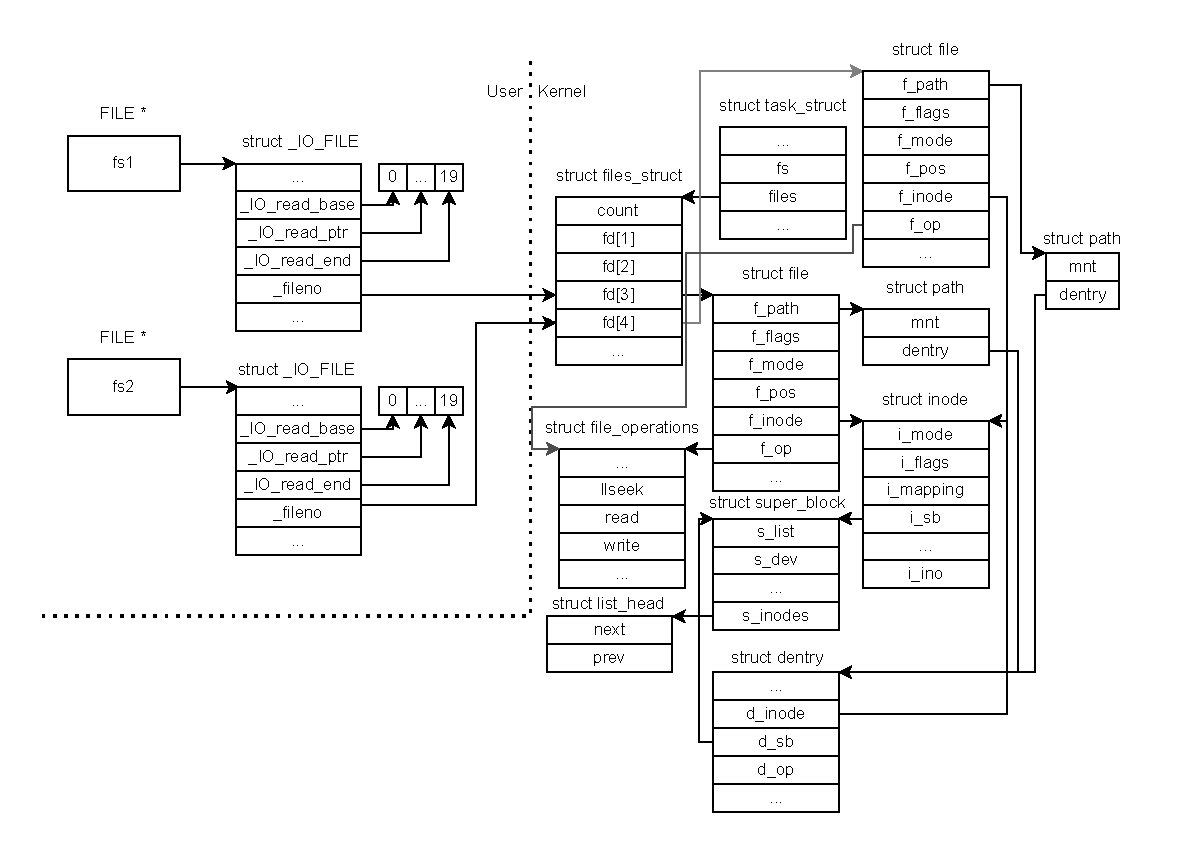
\includegraphics[width=1.1\textwidth]{./img/third.pdf}
	\caption{Связь структур файловой подсистемы Linux}
	\label{fig:323}
\end{figure}
\newpage
